	\documentclass[table,color]{fithesis3/fithesis3}
\usepackage[english]{babel}
\usepackage{amsmath}
\usepackage{tabularx}
\usepackage{booktabs}
\usepackage{graphics}
\usepackage{caption}
\usepackage{subcaption}
\thesissetup{
	faculty=fi,
	title=Adaptive Practice of Facts Using Multiple-Choice Questions,
	type=r,
	author=Jan Papou\v{s}ek,
	advisor=Radek Pel\'{a}nek
}

\begin{document}

\chapter{Introduction}
Using of computers and other electronic devices becomes more and more common in
the educational process. This allows

\begin{itemize}
	\item	wide usage of computers $\rightarrow$ help teachers with routine tasks
				and provide personalized approach for students;
	\item	teacher's aspect vs. student's aspect;
	\item	providing content, complex exercises vs. practicing atomic tasks;
	\item	domains where you need to learn facts -- vocabulary, anatomy, \ldots;
	\item	fixed amount of time at school vs. online environment with a lot of
				possible activities and high fluctuation;
	\item	the system providing practice needs to attract and keep the attention
				of users and spend the given amount of time in the most effective way
				with respect to learning;
	\item	different users have different background - not only knowledge, but
				also the motivation of the practice can differ (vs. school where the
				motivation is $\pm$ the same);
	\item	systems motivating users to stay active $\neq$ systems effective in
				learning;
	\item	there is no obvious technique for practicing in online environment;
	\item	to build a good adaptive you need at least:
		\begin{itemize}
			\item	a good model describing the user's knowledge;
			\item	good strategy for practicing -- may differ for different types of
						users (some users want to learn for the tommorrow exam, some users want to
						learn in long term);
		\end{itemize}
	\item	we can't design a good strategy for practice when we can not measure
				its impact on the user's motivation to practice and the effectivenes for
				learning -- big methodological issue in online environment;
	\item	when we build a widely used system for practice
\end{itemize}

\section{Systems}

\begin{itemize}
	\item Cerego
	\item Duolingo~\cite{von2013duolingo, garcia2013learning}
	\item Fact and Concept Training~\cite{pavlik2007fact,pavlik2008using}
\end{itemize}

\paragraph{literature}

\begin{itemize}
	\item self-testing is an effective strategy that may boost student
		performance~\cite{bjork2013self}
	\item high performers may not need to use repetition and low performers may
		not be motivated~\cite{bjork2013self}
	\item overconfidence~\cite{bjork2013self, kornell2008optimising}
	\item learning process involves making continual assesment and decisions, such
	as what should be studied next and how it should be studied, whether the
	learning that will support later access to some information, concept or
	procedure has been achieved, whether what one has recalled is correct, and so
	on and on~\cite{bjork2013self}
	\item inner vs. outer loop~\cite{koedinger2013new}
\end{itemize}

\chapter{State of the Art}

Development a fully adaptive system providing a practice of facts requires
insights from a few from the first point of view different areas. This chapter
describes state of the art in these areas starting from psychology and
cognitive science to student modelling, controlling the practice itself,
evaluation and concrete systems.

\section{Memory and Learning of Facts}

The common way to learn facts whether online or offline is using
flashcards~\cite{kornell2008optimising}. A flashcard has two sides, the first
side represents a given term we want to learn and the second one its
explanation, e.g. translation or image describing it.  During one practice
session a sequence of flashcards is presented, so firstly we look at one side
trying to say what is on the second side and then check whether our answer is
correct. This really simple setup has a few parameters needed to be considered:

\begin{enumerate}
	\item How many flashcards should be available in one practice session?
	\item What is their optimal order?
	\item Should we drop some flashcards out of the practice if we think we already know it?
	\item Should we gradually add flashcards with new terms and how?
	\item How many time should we repeat the practice?
	\item What is the optimal time space between individual presentations of one flashcard?
\end{enumerate}

\subsection{Spacing Effect}
\label{section:spacing_effect}
ll of the mentioned questions relate to the \emph{spacing
effect} and \emph{forgetting curves} originally discovered by Hermann
Ebbinghaus~\cite{ebbinghaus1885spacing}~(as cited
in~\cite{pavlik2005practice}). When the terms are practiced with more time
space between individual presentations, it reduces our performance during the
practice itself, but in long term it has a positive impact on our
learning~\cite{maass2015how, kornell2009optimising}. This is in the opposite of
usual preparation of students before exams when they prefer \emph{massed
repetition} (also known as \emph{cramming}), intensive work to absorb large
volume of knowledge in short time period.

\begin{figure}
	\begin{center}
		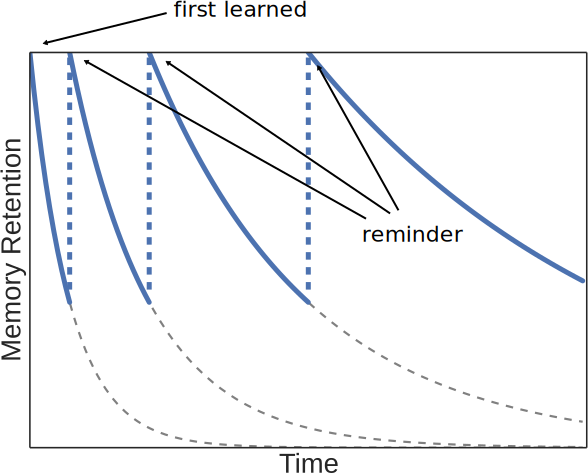
\includegraphics[width=.6\textwidth]{figure/forgetting_curves}
		\caption{Forgetting curve introduced by Ebbinghaus is given by a
			formula $R = e^{-\frac{t}{S}}$, where $R$ stands for the memory retention, $t$
			for the time and $S$ for the relative strength of memory. Ebbinghaus
			found realized that when the information is reminded again, it strengthens
			not only the memory, but also also reduces the forgetting rate. This phenomenon
			is called \emph{overlearning}.
			\textbf{TODO}}
	\end{center}
\end{figure}

In the context of computerized adaptive practice we should look at the spacing
effect from two different points of view. In the first case we want to control
it within one session. Here we have full control over it and we work with
seconds, minutes or hours (maximally). With a fixed number of items for
practice we regulate the spacing by modifying the sequence of practiced items,
e.g. more blocking or iterleaving version of
practice~\cite{ostrow2015blocking}, with variable set of items we can also
decide which items do not have to be practiced
anymore~\cite{kornell2008optimising} or which new items can be included.
Current research shows that in this specific case lies great potential, because
the sequencing has a big impact of the learning
performance~\cite{ostrow2015blocking} and people are not able effectively judge
which items are already learned~\cite{kornell2008optimising} and which ones
should be practiced~\cite{kornell2014focusing}.

In the second case we plan the practice over more
sessions~\cite{kang2014retrieval}. Ideally a system should decide when the
session starts and when it ends. Of course this decision is made by a user,
not by a system. We can only motivate users to practice regularly, e.g. every
day similarly how it is done by Duolingo (a system for learning
languages)~\cite{garcia2013learning}. This regularity allows us to strengthen
knowledge of already learned items and itroduce new ones.

\subsection{Models Overview}

\paragraph{Rasch Model} is known as the one-parameter logistic model in item
response theory (\textbf{TODO: CITE}). It assumes the student's knowledge about
an item is constant and can be expressed as a skill parameters $\theta$. Also
each item is assigned by a difficulty parameter $b$. Having these parameters
the probability of correct answer is given by the logistic function:

\begin{align}
P(correct|\theta,b) = \frac{1}{1 + e^{-(\theta - b)}}
\end{align}

Parameters of this model are usually estimated from data using the joint
maximum likelihood estimation~\cite{de2008theory}. In online environment it is
useful to update the parameters on the fly. For this purpose we can inspire by
Elo rating system~\cite{elo1978rating} originally devised for chess rating and
look at a student's answer on an item as match between the student and
the item~\cite{papousek2014adaptive}. If our estimation is based only on the
first interactions between students and items, the algorithm works for constant
skills and difficulties, although the original Elo system assumes learning (changing skill).

\paragraph{Bayesian Knowledge Tracing} is usually used model for
learning~\cite{van2013properties}. It models student's knowledge in a hidden
Markov model as a binary latent variable (either learned or unlearned). The model
has four parameters: probability the given is initially learned, probability of
learning based on one step, probability of wrong answer when the skill is
learned (slip), and probability of correct answer when the skill is not learned
(guess). Skill estimation is updated using a Bayes rule using observed answer.
Several extensionis of this model can be found, e.g.
forgetting~\cite{qiu2010does} or slightly different point of view using mixture
of learning curves~\cite{streeter2015mixture}.

\paragraph{Performance Factor Analysis} is another logistic
model~\cite{pavlik2009performance}, but in contrast with the Rasch model it
handles learning. The skill is represented as a linear combination of the
item's difficulty ($\beta$) and the number of past success ($s$) and failures
($f$) of the given student.

\begin{align}
P(correct|\beta,s, f) = \frac{1}{1 + e^{-(\beta + \gamma s + \delta f)}}
\end{align}

where $\gamma$ stands for the change of the skill associated with correct
answer and $\delta$ stands for the same in case of incorrect answer.

\bigskip

\noindent
In many areas of learning of facts people enter the tutoring system with varied
prior knowledge, e.g. vocabulary or geography. A system needs to quickly assess
what a user knows to be able to adaptively provide appropriate content. This
feature is often missing in several systems and the user is forced to go through
a lot of useless content. Our recent work~\cite{papousek2014adaptive} simlarly
to~\cite{khajah2014integrating} combines a model assuming a constant skill with
another one for learning to handle this phenomenon.  But this should go even
further and models should also provide different
learning~\cite{pelanek2015modeling} and forgetting rate for different items.
A model using a mixture of individual learning curves implememted within
Duolingo~\cite{streeter2015mixture} already covers some of these aspects, but
they do not give much attention to prior knowledge and ignore spacing effect.
On the other side studies dealing with spacing effect are usually based on
observations in laboratory with artifical conditions, e.g.  people learn
generally uknown terms to prevent prior knowledge~\cite{kang2014retrieval} or
there is no corrective-feedback given during retriaval
practice~\cite{landauer1978optimum}~(as cited in~\cite{kang2014retrieval}) and
it is questionable how all their insights will work within an online system.

\section{Practice Control}

As we already presented in the previous sections we focus on \emph{inner loop}
of user's practice~\cite{koedinger2013new}, mainly within one session, that
is sequencing of items presented to a user. The considered area of learning
of facts doesn't provide sufficiently complex tasks to deal with \emph{outer
loop} (e.g. hints)~\cite{koedinger2013new} and we think it is enough. The
practice itself consists of a sequence of multiple-choice and open-ended
questions and we have to decide not only which item should be practiced, but
also whether and how many options the question should have and in case of
multiple-choice questions which items should be used as distractors. Sequencing
should also take into account spacing effect described in
section~\ref{section:spacing_effect}.

\subsection{Sequencing}

By seqencing the items presented to a user for practice we balance between two
states: \emph{over-practice} and \emph{under-practice}. In the first case we
practice an already learned item and we waste user's time. In the second one we
stop practicing an item which is not learned yet and we will not give her a
chance learn it completely. When a system tries to avoid over-practiced
attempts, there is high chance that under-practice increases and vice versa.
How this phenomenon is importent is presented in a study~\cite{cen2007over}
where its authors reported that analysing historical data they detected more
than $50\%$ out of practice attempts as over-practiced.

In a lot of used systems a general approach for sequencing the items for
practice is based on labelling from an expert. The experts defines knowledge
components for the given domain and prerequisites among them. There are
techniques helping the ex\-perts~\cite{niznan2014using} or completely replace
them by a computer~\cite{boros2013automatic}. However, these techniques are
rarely used. Each component is a set of items and generally one item can be
included within more components. We can practice items belonging to one
component as long as the given user has mastered its prerequisites, but not the
component itself. This edge of knowledge is also known as the \emph{zone of
proximal development}~\cite{lee2005signifying}.

The mastery is detected by a model predicting user's performance and we say
that the user masters the knowledge component when the predicted probability
the user learned the component exceeds the \emph{mastery threshold} which is
usually set to~$95\%$. Mastery threshold can be viewed as parameter controlling
the relative frequency of under-practiced and over-practiced
attempts~\cite{fancsali2013optimal}. Since our model needs data about a user
to make estimation, there is some low acceptable number of attempts after the
enowledge is acquired. This \emph{lag} studied in more detail
in~\cite{fancsali2013optimal}, but the study is limited for \emph{Bayesian
knowledge tracing} only.

Similar approach is presented in~\cite{lopes2015multi}, where the system relies
on~\emph{multi-armed bandits}, a technique generally being able to explore
space of different parameters or strategies with respect to a given scoring
function. The authors define a structure of activites and pre-conditions
analogical to knowledge components and prerequisites and introduce two
algorithms optimizing user's learning. The first one is independent on any
model estimating user's performance, the second one uses it. Both of them take
information from experts and measure user's learning online based on progress
of the user's performance. The exact measure is defined as:

\begin{align}
	r = \sum^{t}_{k = t - \frac{d}{2}} \frac{C_k}{\frac{d}{2}} - \sum^{t - \frac{d}{2}}_{k = t - d} \frac{C_k}{d - \frac{d}{2}}
\end{align}

where $C_k = 1$ if the exercise at time $k$ was solved correctly. At time $t$,
the measure compares the success of the last $\frac{d}{2}$ samples with the
$\frac{d}{2}$ previous samples. Learning can estimated by this way thanks to
the fact, the system measures and improves the user's performance at the same
time. We show in section~\ref{section:evaluation} this is not always true in
some kind of systems.

In some cases the approach using a graph of prerequisites makes sense, e.g.
in algebra we have a strong structure of prerequisites among the knowledge
components (addition and multiplication) and the choice of an item (exercise)
from the knowledge component is not so important, if we know that all
prerequisites for the given component are mastered. On the other hand in case
of a system for learning of vocabulary, individual items are independent, so we
have one item per knowledge component. Of course we can build a structure of
categories and prerequisites, but they represent a recommended study plan
rather than necessity. When a user enters the system, she can theoretically
start practicing anything.

In~\cite{papousek2014adaptive} and~\cite{papousek2015impact} we present an
approach mainly based on target difficulty. We assume we have already
estimation of user's performance for each item available in our system,
together with other descriptive information like number of interactions with
the given item, last time when the user interacted with it and so on. Since the
estimation is based only on historical data we do not need any expert's input.
On the other side we are fully dependent on the choice of target difficulty and
although there are studies about it~\cite{lomas2013optimizing,
lomas2014optimizing,jansen2013influence,papousek2015impact}, further research
has to be done in this area. Several systems has this parameter set
arbitrarily, e.g.  75\% chance of correct
answer~\cite{klinkenberg2011computer}.

As we present in section~\ref{section:spacing_effect}, learning of facts highly
releates to time and spacing effect. From this point of view the  schedule of
practice was already studied~\cite{pavlik2008schedule}, but in different
context, which is in laboratory with low number of items and without any prior
knowledge. Figure~\ref{figure:practice_progress} shows how the spacing effect
relates to the content of practice and number of practiced items.

\begin{figure}
	\begin{subfigure}[b]{.5\textwidth}
		\centering
		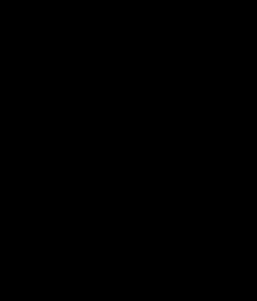
\includegraphics[width=0.9\textwidth]{figure/practice_progress_a}
		\caption{high spacing}
		\label{figure:practice_progress_a}
	\end{subfigure}
	\begin{subfigure}[b]{.5\textwidth}
		\centering
		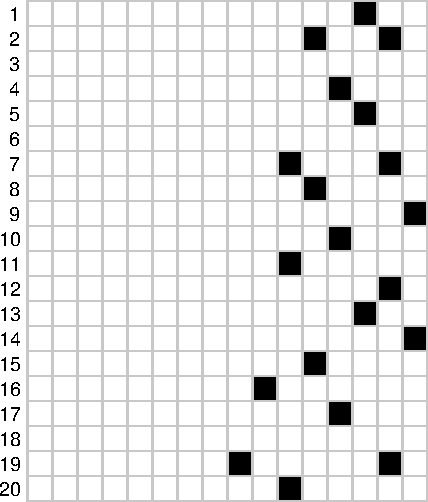
\includegraphics[width=0.9\textwidth]{figure/practice_progress_b}
		\caption{low spacing}
		\label{figure:practice_progress_b}
	\end{subfigure}
	\caption{Visualization of practice with different spacing, each column
		corresponds to an item, each row represents a discrete time unit. Black
		boxes stands for practice attempts.}
	\label{figure:practice_progress}
\end{figure}

\subsection{Questions}

Assume we have already picked an item for practice which correspons to a
flashcard with two sides $A$ and $B$. We must specify a direction of the final
question (whether we ask for the side $A$ or $B$), e.g. in case of vocabulary
the first direction leads to an ability of understanding to foreign language
and the second one to an ability of expressing of ideas in it. In both ways we
want to achieve so-called \emph{cued recall}~(\textbf{TODO: cite}).

Once we select a direction we must decide whether the question will be
open-ended or how many options it will have. Using the options we allow a user
to guess the correct answer, so we make the question easier.
Figure~\ref{figure:options_vs_spacing} shows how the number of options relates
to difficulty of the final question together with spacing which is controlled
by sequencing. If our only goal is to make the difficulty of user's practice
appropriate, it is not clear which combination of spacing and number of options
we should use.

\begin{figure}[h]
	\begin{center}
		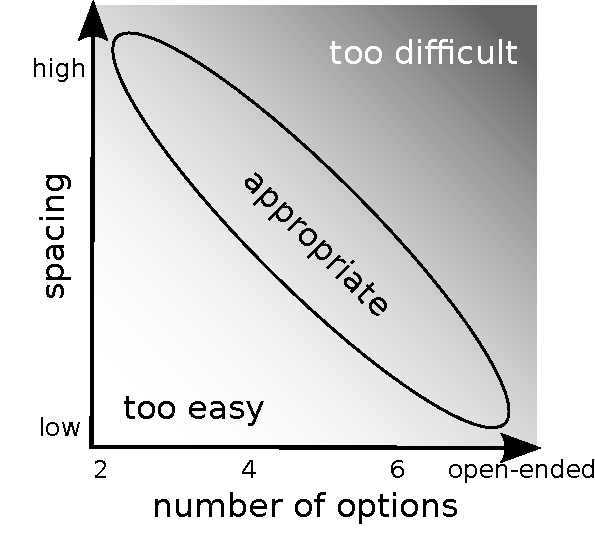
\includegraphics[width=.5\textwidth]{figure/options_vs_spacing}
	\end{center}
	\caption{Graph illustrating how difficulty depends on spacing and number of
		options. Darker background color means more difficult practice.}
	\label{figure:options_vs_spacing}
\end{figure}

The next issue is how exactly should be the options themselves be chosen. We
assume too easy options made the guess probability so high, a user wouldn't be
motivated to learn anything. The impact of competitivness of options has been
studied in~\cite{little2015optimizing}. The study contains two experiments
where the first one does not include feedback about the correctness of user's
answer, so its results can be hardly applied within an application where the
feedback is present. And based on the second experiment where the feedback was
included, competitive options seem to be the better choice. However the
experiment was very limited, so this phenomenon is worth further investigation.

The second aspect related to the competitivness of the options is repeating the
same mistakes. Authors in~\cite{marsh2007memorial} describe experiments where
wrong answer in the final test are correlated to wrong answer within a
preparation phase where multiple-choice question were used. These observation
should be definitely taken into account when the options are built within an
adaptive system for practice.

\section{Evaluation}
\label{section:evaluation}

\begin{itemize}
	\item only student model and its accuracy~\cite{pelanek2014brief}
	\item saved time for getting mastery~\cite{yudelson2015small}
	\item combination of historical data and simulation~\cite{gonzalez2015your}
	\item exploring the interaction loop using synthetic data~\cite{niznan2015exploring}
	\item learning vs. time spent in a system~\cite{lomas2013optimizing, monterrat2015player},
	\item online multivariate (AB) testing~\cite{lomas2013optimizing,liu2014towards,stamper2012rise}
	\item multi-armed bandits~\cite{liu2014trading,lopes2015multi}
	\item recommender systems: model performance vs. impact~\cite{cremonesi2010performance}
	\item debugging/tunning techniques for adaptive learning systems
		\begin{itemize}
			\item system behavior is hard to predict
			\item it is easy to make a mistake
			\item it is difficult to tune parameters of practice
			\item how can we make it easier?
		\end{itemize}
	\item appropriate measures of user's progress
		\begin{itemize}
			\item success
			\item coverage
			\item diversity~\cite{lopes2015multi}
		\end{itemize}
\end{itemize}

\chapter{Aims of the Thesis}

The main aim of the thesis is to design and evaluate several techniques of
learning of factographical knowledge via practice of multiple choice questions in
online environment. Although the work is focused on the practice of geography,
the found results will be easily appliable to other similar domains like
vocabulary.

\begin{itemize}
	\item canary deployment in the context of ITS
\end{itemize}

\section{Objectives}

\begin{itemize}
	\item deploy a system used for \url{http://slepemapy.cz} with data for
		anatomy to get more historical data about one user;
	\item propose a methodology to evaluate the impact of adaptive practice on
		student's learning in online environment;
	\item implement the proposed methodology within a system for adaptive
		practice of geography and anatomy;
	\item design and implement a model of forgetting (cooperating with model for
		estimation of prior knowledge)
	\item find optimal parameters of adaptive practice with respect to motivation
		and learning (it can differ for different groups of users)
		\begin{itemize}
			\item target difficulty;
			\item spacing
			\item choice of distractors
			\item recall vs. recognition
		\end{itemize}
\end{itemize}

\section{Proposed Plan of Work}

\section{Future Publications}

\chapter{Achieved results}

\begin{itemize}
	\item system for adaptive practice of geography~\cite{papousek2014adaptive}
	\item evaluation of the system with respect to user's motivation~\cite{papousek2015impact}
	\item feedback loop~\cite{niznan2015exploring}
	\item analysis of response time~\cite{papousek2015analysis}
\end{itemize}

\bibliographystyle{plain}
\bibliography{proposal}
\end{document}
